\documentclass[12pt]{article}

\usepackage[margin=1in]{geometry}

%For 3D plots
\usepackage{blindtext}
\usepackage{pgfplots}
\pgfplotsset{compat=1.9}
% For inline color changes
\usepackage{xcolor}
% For vertical brace rcases
\usepackage{mathtools}
% For positioning figures
\usepackage{float}
% makes figure font bold
\usepackage{caption}
\captionsetup[figure]{labelfont=bf}
% For text generation
\usepackage{lipsum}
% For drawing
\usepackage{tikz}
% For manipulating coordinates
\usetikzlibrary{calc}
% For relative node positioning
\usetikzlibrary{positioning}
% For smaller or equal sign and not divide sign
\usepackage{amssymb}
% For the diagonal fraction
\usepackage{xfrac}
% For enumerating exercise parts with letters instead of numbers
\usepackage{enumitem}
% For dfrac, which forces the fraction to be in display mode (large) e
% even in math mode (small)
\usepackage{amsmath}
% For degree sign
\usepackage{gensymb}
% For "\mathbb" macro
\usepackage{amsfonts}
\newcommand{\nbb}{\mathbb{N}}
\newcommand{\zbb}{\mathbb{Z}}
\newcommand{\qbb}{\mathbb{Q}}
\newcommand{\rbb}{\mathbb{R}}
\newcommand{\cbb}{\mathbb{C}}
\newcommand{\fbb}{\mathbb{F}}
\newcommand{\rad}{\text{ rad}}
\newcommand{\lcm}{\text{lcm}}
\newcommand{\Aut}{\text{Aut}}
\newcommand{\seq}{\leqslant}
\newcommand{\beq}{\geqslant}
\newcommand{\sub}{\subseteq}
\newcommand{\prosub}{\subset}

\newcommand{\Ocal}{\mathcal{O}}
\newcommand{\cbbcal}{\mathcal{C}}
\newcommand{\Pcal}{\mathcal{P}}
\newcommand{\Scal}{\mathcal{S}}

% overline short italic
\newcommand{\olsi}[1]{\,\overline{\!{#1}}}

\title{%
    \Huge Abstract Algebra \\
    \large by \\
    \Large Dummit and Foote \\~\\
    \huge Part 1: Group Theory \\
    \LARGE Chapter 2: Subgroups \\
    \Large Section 5: The Lattice of Subgroups of a Group
}
\date{2023-07-14}
\author{Michael Saba}

\begin{document}
    \pagenumbering{gobble}
    \maketitle
    \newpage
    \pagenumbering{arabic}


    \section*{Exercise 1}
    For $\{1\} \seq H, K \seq G$,
    (there can be other subgroups)
    the possible sublattices of $G$ containing only these groups are:

    \begin{figure}[H]
        \centering
        % figure is a tikz drawing
        \begin{tikzpicture}[scale=2.5]

        \def\d{.7cm}

        % Specifies where the x, y coordinate of the tip of
        % the unite vectors in turn
        \tikzset{}
        
        % Scope used to shift the coordinates from the basis
        \begin{scope}[shift={(0, 0, 0)}, rotate=0]
            \node (G1) at (0, 0) {$G$};   
            \node (H1) [below left=\d and \d of G1] {$H$};   
            \node (K1) [below right=\d and \d of G1] {$K$};   
            \node (T1) [below right=\d and \d of H1] {$\left\{ 1 \right\}$}; 
            
            \node (G2) at (2, 0) {$G$};   
            \node (H2) [below left=\d and \d of G2] {$H$};   
            \node (K2) [below left=\d and \d of H2] {$K$};   
            \node (T2) [below left=\d and \d of K2] {$\left\{ 1 \right\}$}; 

            \node (G3) at (3, 0) {$G$};   
            \node (K3) [below left=\d and \d of G3] {$K$};   
            \node (H3) [below left=\d and \d of K3] {$H$};   
            \node (T3) [below left=\d and \d of H3] {$\left\{ 1 \right\}$}; 
        \end{scope}

        \begin{scope}[thick]
            \draw (G1) -- (H1);
            \draw (G1) -- (K1);
            \draw (K1) -- (T1);
            \draw (H1) -- (T1);

            \draw (G2) -- (H2);
            \draw (H2) -- (K2);
            \draw (K2) -- (T2);

            \draw (G3) -- (K3);
            \draw (K3) -- (H3);
            \draw (H3) -- (T3);
        \end{scope} 

        \end{tikzpicture}

        \caption{\label{fig:figure1} Possible sublattices of the group $G$.}
    \end{figure} 

    The sublattices are distinguished by the inclusions
    of $H$ and $K$. While it's always the case that $\{1\}$
    is contained in all subgroups and $G$ contains all subgroups,
    $H$ and $K$ can contain one another or not.


    \section*{Exercise 2}
    Going by the lattice of $D_{16}$: 

    \begin{figure}[H]
        \centering
        % figure is a tikz drawing
        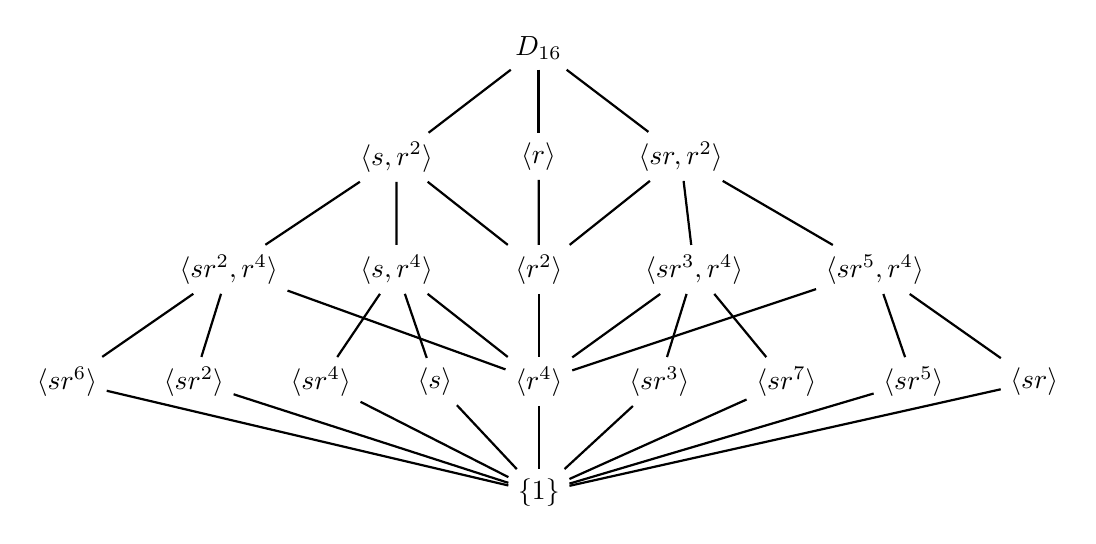
\begin{tikzpicture}[scale=2.5]

        \def\d{.8cm}
        \def\h{.6cm}

        % Specifies where the x, y coordinate of the tip of
        % the unite vectors in turn
        \tikzset{}
        
        % Scope used to shift the coordinates from the basis
        \begin{scope}[shift={(0, 0, 0)}, rotate=0]
            \node (D16) at (0, 0) {$D_{16}$};   
            \node (A1) [below left=\d and \d of D16]
            {$\langle s, r^2 \rangle$}; 
            \node (A2) [below= \d of D16] {$\langle r \rangle$}; 
            \node (A3) [right= \d of A2]
            {$\langle sr, r^2 \rangle$};  
            \node (B1) [below left=\d and \d of A1]
            {$\langle sr^2, r^4 \rangle$}; 
            \node (B2) [right=\d of B1] {$\langle s, r^4 \rangle$}; 
            \node (B3) [right=\d of B2]
            {$\langle r^2 \rangle$};  
            \node (B4) [right=\d of B3] {$\langle sr^3, r^4 \rangle$}; 
            \node (B5) [right=\d of B4]
            {$\langle sr^5, r^4 \rangle$};  

            \node (C1) [below left=\d and \d of B1]
            {$\langle sr^6 \rangle$}; 
            \node (C2) [right= \h of C1]
            {$\langle sr^2 \rangle$}; 
            \node (C3) [right= \h  of C2]
            {$\langle sr^4 \rangle$}; 
            \node (C4) [right= \h of C3]
            {$\langle s \rangle$}; 
            \node (C5) [below= \d of B3] {$\langle r^4 \rangle$};
            \node (C6) [right= \h of C5]
            {$\langle sr^3 \rangle$}; 
            \node (C7) [right= \h of C6]
            {$\langle sr^7 \rangle$};
            \node (C8) [right= \h of C7]
            {$\langle sr^5 \rangle$};  
            \node (C9) [right= \h of C8]
            {$\langle sr \rangle$};  
            
            \node (T1) [below=\d of C5] {$\left\{ 1 \right\}$}; 
        \end{scope}

        \begin{scope}[thick]
            \draw (D16) -- (A1);
            \draw (D16) -- (A2);
            \draw (D16) -- (A3);
            \draw (A1) -- (B1);
            \draw (A1) -- (B2);
            \draw (A1) -- (B3);
            \draw (A3) -- (B5);
            \draw (A3) -- (B4);
            \draw (A3) -- (B3);
            \draw (A2) -- (B3);
            \draw (B3) -- (C5);
            \draw (B1) -- (C1);
            \draw (B1) -- (C2);
            \draw (B1) -- (C5);
            \draw (B2) -- (C3);
            \draw (B2) -- (C4);
            \draw (B2) -- (C5);
            \draw (B4) -- (C6);
            \draw (B4) -- (C7);
            \draw (B4) -- (C5);
            \draw (B5) -- (C8);
            \draw (B5) -- (C9);
            \draw (B5) -- (C5);

            \foreach\x in {1,..., 9}
            \draw (C\x) -- (T1);
        \end{scope} 

        \end{tikzpicture}

        \caption{\label{fig:figure1} Lattice of $D_{16}.$}
    \end{figure} 

    \begin{enumerate}[label=\textbf{\alph*.}]
        \item 
            We have \[ \langle sr^2, r^4 \rangle
            \beq \langle sr^2, r^4 \rangle, \langle sr^6 \rangle,
            \langle sr^2 \rangle, \langle r^4 \rangle, \{1\} \]
        \item 
            We have \[ \langle sr^7, r^4 \rangle = \langle sr^3, r^4 \rangle 
            \beq \langle sr^3, r^4 \rangle, \langle sr^3 \rangle,
            \langle sr^7 \rangle, \langle r^4 \rangle, \{1\} \]
        \item 
            We have         
            \begin{align*}
                \langle r^4 \rangle
                \seq \langle r^4 \rangle, \langle sr^2, r^4 \rangle,
                \langle s, r^4 \rangle, \langle sr^3, r^4 \rangle,
                \langle sr^5, r^4 \rangle, \langle r^2 \rangle,
                \langle r \rangle, \langle s, r^2 \rangle, \\
                \langle sr, r^2 \rangle, \langle r \rangle, D_{16}
            \end{align*}
        \item 
            We have \[ \langle s \rangle
            \seq  \langle s \rangle, \langle s, r^4 \rangle,
            \langle s, r^2 \rangle, D_{16} \]
    \end{enumerate}


    \section*{Exercise 3}
    Proof that in $D_8$, $\langle s, r^2 \rangle \cong V_4$
    (\textit{the Klein 4-Group}): \\
    We can probe that $\langle s, r^2 \rangle \cong V_4$
    by drawing their group tables:

    \begin{figure}[H]
        \centering

        \[\vbox{\tabskip0.5em\offinterlineskip
        \halign{\strut$#$\hfil\ \tabskip1em\vrule&&$#$\hfil\cr
        ~   & 1   & a   & b & c \cr
        \noalign{\hrule}\vrule height 12pt width 0pt
        1   & 1 & a & b & c \cr 
        a   & a & 1 & c & b \cr 
        b   & b & c & 1 & a \cr 
        c   & c & b & a & 1 \cr
        }}\]

        
        \[\vbox{\tabskip0.5em\offinterlineskip
        \halign{\strut$#$\hfil\ \tabskip1em\vrule&&$#$\hfil\cr
        ~   & 1   & s   & r^2 & sr^2 \cr
        \noalign{\hrule}\vrule height 12pt width 0pt
        1   & 1 & s & r^2 & sr^2 \cr 
        s   & s & 1 & sr^2 & r^2 \cr 
        r^2   & r^2 & sr^2 & 1 & s \cr 
        sr^2   & sr^2 & r^2 & s & 1 \cr
        }}\]

        \caption{\label{fig:figure1} The group tables of $V_4$
        and $\langle s, r^2 \rangle$.}
    \end{figure}

    By mapping $a$ to $s$, $b$ to $r^2$, and $c$ to $sr^2$,
    the tables are equivalent,
    so the groups are isomorphic. \\ 
    Alternatively, we can refer to a later proof in exercise 1.2.5.10
    which states that there are only two unique groups of order 4,
    the cyclic group $Z_4 = \langle x \rangle$,
    and the non-cyclic Klein 4-Group $V_4 = \{1, a, b, c\}$.
    This means that $\langle s, r^2 \rangle$
    is isomorphic to one of them.
    Since it is by deifnition not generated by a single element,
    it can't be isomorphic to $Z_4$,
    so it is isomorphic to $V_4$.


    \section*{Exercise 4}
    We know that $D_8$ is generated by $r$ and $s$,
    so $D_8 = \langle r, s \rangle$.
    So we need to look at the lattice of $D_8$
    and count all the pairs of elements that aren't equal to 
    any of the proper subgroups of $D_8$.
    If for instance, $\langle x, y \rangle$ where $x, y \in D_8$
    isn't a proper subgroup of $D_8$,
    then, since $D_8$ is closed under inverses and composition,
    this can only mean that $D_8 = \langle x, y \rangle$.
    So, given

    \begin{figure}[H]
        \centering
        % figure is a tikz drawing
        \begin{tikzpicture}[scale=2.5]

        \def\d{.8cm}

        % Specifies where the x, y coordinate of the tip of
        % the unite vectors in turn
        \tikzset{}
        
        % Scope used to shift the coordinates from the basis
        \begin{scope}[shift={(0, 0, 0)}, rotate=0]
            \node (Q8) at (0, 0) {$D_8$};   
            \node (A1) [below left=\d and \d of G1]
            {$\langle s, r^2 \rangle$}; 
            \node (A2) [below= \d of G1] {$\langle r \rangle$}; 
            \node (A3) [below right=\d and \d of G1]
            {$\langle rs, r^2 \rangle$};  
            \node (B1) [below left=\d and \d of A1]
            {$\langle r^2s \rangle$}; 
            \node (B2) [below= \d of A1] {$\langle s \rangle$}; 
            \node (B3) [below=\d of A2]
            {$\langle r^2 \rangle$};  
            \node (B4) [below= \d of A3] {$\langle rs \rangle$}; 
            \node (B5) [below right=\d and \d of A3]
            {$\langle r^3s \rangle$};  
            \node (T1) [below=\d of B3] {$\left\{ 1 \right\}$}; 
        \end{scope}

        \begin{scope}[thick]
            \draw (Q8) -- (A1);
            \draw (Q8) -- (A2);
            \draw (Q8) -- (A3);
            \draw (A1) -- (B1);
            \draw (A1) -- (B2);
            \draw (A1) -- (B3);
            \draw (A3) -- (B5);
            \draw (A3) -- (B4);
            \draw (A3) -- (B3);
            \draw (A2) -- (B3);

            \foreach\x in {1,..., 5}
            \draw (B\x) -- (T1);
        \end{scope} 

        \end{tikzpicture}

        \caption{\label{fig:figure1} Lattice of $D_8.$}
    \end{figure} 

    With that, we have that
    $\langle r, s \rangle$, $\langle r^3, s \rangle$,
    $\langle sr, s \rangle$, $\langle sr^3, s \rangle$,
    $\langle r^3, sr \rangle$, $\langle r^3, sr^3 \rangle$,
    $\langle sr, sr^3 \rangle$, $\langle sr, r \rangle$,
    $\langle sr, r^3 \rangle$, $\langle sr, sr^2 \rangle$,
    $\langle sr^2, r \rangle$, $\langle sr^3, r \rangle$
    are all 12 of the unique pairs of elements that 
    generate all of $D_8$
    instead of being equal to one of its proper subgroups.


    \section*{Exercise 5}
    We need to find all 8 elements $x \in D_{16}$
    such that $\langle x, s \rangle = D_{16}$.
    Like exercise 1.2.5.4, we can do this by finding
    all values of $x$ for which the group $\langle x, s \rangle$
    is not equal to one of the subgroups of $D_{16}$ in its lattice

    \begin{figure}[H]
        \centering
        % figure is a tikz drawing
        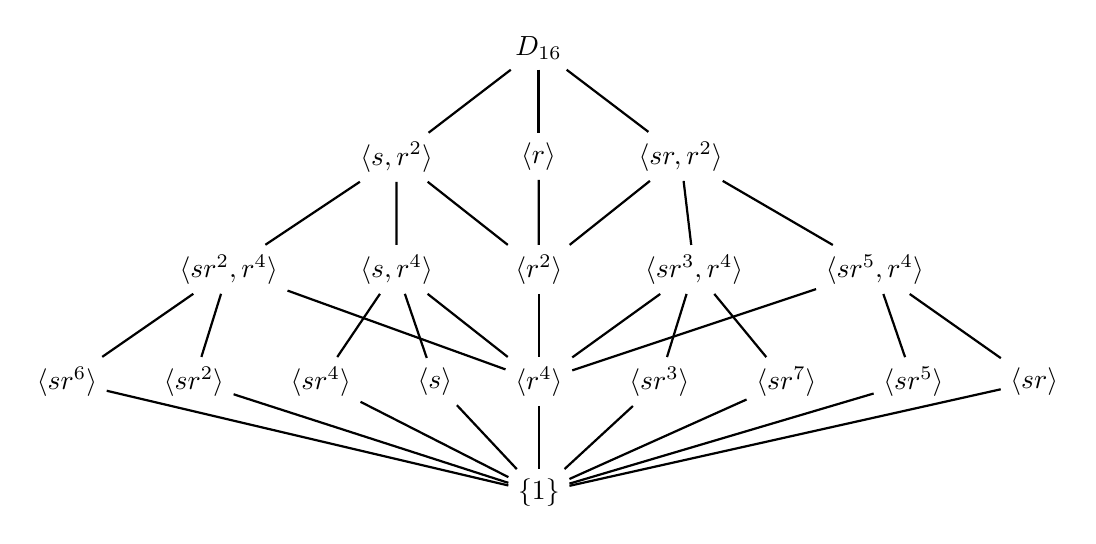
\begin{tikzpicture}[scale=2.5]

        \def\d{.8cm}
        \def\h{.6cm}

        % Specifies where the x, y coordinate of the tip of
        % the unite vectors in turn
        \tikzset{}
        
        % Scope used to shift the coordinates from the basis
        \begin{scope}[shift={(0, 0, 0)}, rotate=0]
            \node (D16) at (0, 0) {$D_{16}$};   
            \node (A1) [below left=\d and \d of D16]
            {$\langle s, r^2 \rangle$}; 
            \node (A2) [below= \d of D16] {$\langle r \rangle$}; 
            \node (A3) [right= \d of A2]
            {$\langle sr, r^2 \rangle$};  
            \node (B1) [below left=\d and \d of A1]
            {$\langle sr^2, r^4 \rangle$}; 
            \node (B2) [right=\d of B1] {$\langle s, r^4 \rangle$}; 
            \node (B3) [right=\d of B2]
            {$\langle r^2 \rangle$};  
            \node (B4) [right=\d of B3] {$\langle sr^3, r^4 \rangle$}; 
            \node (B5) [right=\d of B4]
            {$\langle sr^5, r^4 \rangle$};  

            \node (C1) [below left=\d and \d of B1]
            {$\langle sr^6 \rangle$}; 
            \node (C2) [right= \h of C1]
            {$\langle sr^2 \rangle$}; 
            \node (C3) [right= \h  of C2]
            {$\langle sr^4 \rangle$}; 
            \node (C4) [right= \h of C3]
            {$\langle s \rangle$}; 
            \node (C5) [below= \d of B3] {$\langle r^4 \rangle$};
            \node (C6) [right= \h of C5]
            {$\langle sr^3 \rangle$}; 
            \node (C7) [right= \h of C6]
            {$\langle sr^7 \rangle$};
            \node (C8) [right= \h of C7]
            {$\langle sr^5 \rangle$};  
            \node (C9) [right= \h of C8]
            {$\langle sr \rangle$};  
            
            \node (T1) [below=\d of C5] {$\left\{ 1 \right\}$}; 
        \end{scope}

        \begin{scope}[thick]
            \draw (D16) -- (A1);
            \draw (D16) -- (A2);
            \draw (D16) -- (A3);
            \draw (A1) -- (B1);
            \draw (A1) -- (B2);
            \draw (A1) -- (B3);
            \draw (A3) -- (B5);
            \draw (A3) -- (B4);
            \draw (A3) -- (B3);
            \draw (A2) -- (B3);
            \draw (B3) -- (C5);
            \draw (B1) -- (C1);
            \draw (B1) -- (C2);
            \draw (B1) -- (C5);
            \draw (B2) -- (C3);
            \draw (B2) -- (C4);
            \draw (B2) -- (C5);
            \draw (B4) -- (C6);
            \draw (B4) -- (C7);
            \draw (B4) -- (C5);
            \draw (B5) -- (C8);
            \draw (B5) -- (C9);
            \draw (B5) -- (C5);

            \foreach\x in {1,..., 9}
            \draw (C\x) -- (T1);
        \end{scope} 

        \end{tikzpicture}

        \caption{\label{fig:figure1} Lattice of $D_{16}.$}
    \end{figure} 

    So we have $\langle r, s \rangle$, $\langle r^3, s \rangle$,
    $\langle r^5, s \rangle$, $\langle r^7, s \rangle$,
    $\langle sr, s \rangle$, $\langle sr^3, s \rangle$,
    $\langle sr^5, s \rangle$, $\langle sr^7, s \rangle$,
    none of which are equivalent to any of the proper subgroups
    of $D_{16}$,
    so as $D_{16}$ is closed under composition and inverses,
    that must make them all equal to $D_{16}$.


    \section*{Exercise 6}
    We know that the centralizers of each group are a subgroup
    of that group,
    so they will feature in its lattice.
    We can then look at each subgroup, and for each element
    in the group, find the highest subgroup where all
    of its elements commute with it.
    The reason we go for the highest is because
    we want all elements that commute with the chosen element, not some.
    \begin{enumerate}[label=\textbf{\alph*.}]
        \item 
            For $D_8$,
            we already know that $r^2$ commutes with all other elements:

            \begin{figure}[H]
                \centering
                % figure is a tikz drawing
                \begin{tikzpicture}[scale=2.5]
        
                \def\d{.8cm}
        
                % Specifies where the x, y coordinate of the tip of
                % the unite vectors in turn
                \tikzset{}
                
                % Scope used to shift the coordinates from the basis
                \begin{scope}[shift={(0, 0, 0)}, rotate=0]
                    \node (Q8) at (0, 0) {$D_8$};   
                    \node (A1) [below left=\d and \d of G1]
                    {$\langle s, r^2 \rangle$}; 
                    \node (A2) [below= \d of G1] {$\langle r \rangle$}; 
                    \node (A3) [below right=\d and \d of G1]
                    {$\langle rs, r^2 \rangle$};  
                    \node (B1) [below left=\d and \d of A1]
                    {$\langle r^2s \rangle$}; 
                    \node (B2) [below= \d of A1] {$\langle s \rangle$}; 
                    \node (B3) [below= \d of A2]
                    {$\langle r^2 \rangle$};  
                    \node (B4) [below= \d of A3] {$\langle rs \rangle$}; 
                    \node (B5) [below right=\d and \d of A3]
                    {$\langle r^3s \rangle$};  
                    \node (T1) [below=\d of B3] {$\left\{ 1 \right\}$}; 
                \end{scope}
        
                \begin{scope}[thick]
                    \draw (Q8) -- (A1);
                    \draw (Q8) -- (A2);
                    \draw (Q8) -- (A3);
                    \draw (A1) -- (B1);
                    \draw (A1) -- (B2);
                    \draw (A1) -- (B3);
                    \draw (A3) -- (B5);
                    \draw (A3) -- (B4);
                    \draw (A3) -- (B3);
                    \draw (A2) -- (B3);
        
                    \foreach\x in {1,..., 5}
                    \draw (B\x) -- (T1);
                \end{scope} 
        
                \end{tikzpicture}
        
                \caption{\label{fig:figure1} Lattice of $D_8.$}
            \end{figure} 

            $C_{D_8}(\{1\}) = D_8$, \\
            $C_{D_8}(\{r\}) = \langle r \rangle$, \\
            $C_{D_8}(\{r^2\}) = D_8$, \\
            $C_{D_8}(\{r^3\}) = \langle r \rangle$, \\
            $C_{D_8}(\{s\}) = \langle s, r^2 \rangle$, \\
            $C_{D_8}(\{sr\}) = \langle rs, r^2 \rangle$, \\
            $C_{D_8}(\{sr^2\}) = \langle s, r^2 \rangle$, \\
            $C_{D_8}(\{sr^3\}) = \langle rs, r^2 \rangle$.
        \item 
            For $Q_8$,
            we know that 1 and $-1$ commute with all other elements,
            and every imaginary number $i$, $j$, and $k$
            only commute with the reals and themselves:

            \begin{figure}[H]
                \centering
                % figure is a tikz drawing
                \begin{tikzpicture}[scale=2.5]
        
                \def\d{.5cm}
        
                % Specifies where the x, y coordinate of the tip of
                % the unite vectors in turn
                \tikzset{}
                
                % Scope used to shift the coordinates from the basis
                \begin{scope}[shift={(0, 0, 0)}, rotate=0]
                    \node (Q8) at (0, 0) {$Q_8$};   
                    \node (A1) [below left=\d and \d of G1]
                    {$\langle i \rangle$}; 
                    \node (A2) [below= \d of G1] {$\langle j \rangle$}; 
                    \node (A3) [below right=\d and \d of G1]
                    {$\langle k \rangle$};  
                    \node (B3) [below= \d of A2]
                    {$\langle -1 \rangle$};  
                    \node (T1) [below=\d of B3] {$\left\{ 1 \right\}$}; 
                \end{scope}
        
                \begin{scope}[thick]
                    \draw (Q8) -- (A1);
                    \draw (Q8) -- (A2);
                    \draw (Q8) -- (A3);
                    \draw (A1) -- (B3);
                    \draw (A3) -- (B3);
                    \draw (A2) -- (B3);
                    \draw (B3) -- (T1);
                \end{scope} 
        
                \end{tikzpicture}
        
                \caption{\label{fig:figure1} Lattice of $Q_8.$}
            \end{figure} 

            $C_{Q_8}(\{1\}) = Q_8$, \\
            $C_{Q_8}(\{-1\}) = Q_8$, \\
            $C_{Q_8}(\{i\}) = \langle i \rangle$, \\
            $C_{Q_8}(\{-i\}) = \langle i \rangle$, \\
            $C_{Q_8}(\{j\}) = \langle j \rangle$, \\
            $C_{Q_8}(\{-j\}) = \langle j \rangle$, \\
            $C_{Q_8}(\{k\}) = \langle k \rangle$, \\
            $C_{Q_8}(\{-k\}) = \langle k \rangle$.

        \item
            For $S_3$,
            we know that every permutation commutes with another
            permutation if and only if they are disjoint,
            or if each cycle in their cycle decomposition
            permutes the same elements (order notwithstanding):

            \begin{figure}[H]
                \centering
                % figure is a tikz drawing
                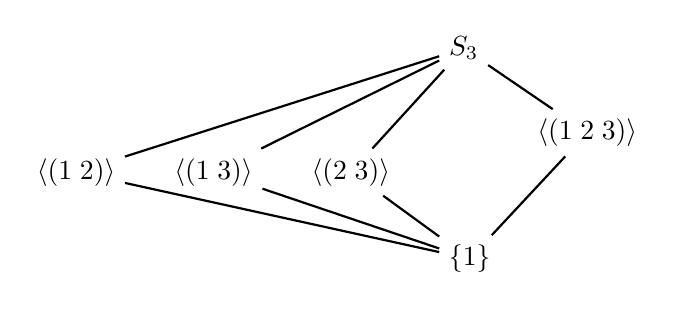
\begin{tikzpicture}[scale=2.5]
        
                \def\d{.5cm}
        
                % Specifies where the x, y coordinate of the tip of
                % the unite vectors in turn
                \tikzset{}
                
                % Scope used to shift the coordinates from the basis
                \begin{scope}[shift={(0, 0, 0)}, rotate=0]
                    \node (S3) at (0, 0) {$S_3$};   
                    \node (A1) [below right=\d and \d of S3]
                    {$\langle (1\;2\;3) \rangle$}; 
                    \node (B1) [below left= 2 * \d and \d of S3]
                    {$\langle (2\;3) \rangle$}; 
                    \node (B2) [left= \d of B1]
                    {$\langle (1\;3) \rangle$};  
                    \node (B3) [left= \d of B2]
                    {$\langle (1\;2) \rangle$};  

                    \node (T1) [below right=\d and \d of B1]
                    {$\left\{ 1 \right\}$}; 
                \end{scope}
        
                \begin{scope}[thick]
                    \draw (S3) -- (A1);
                    \draw (S3) -- (B1);
                    \draw (S3) -- (B2);
                    \draw (S3) -- (B3);
                    \draw (A1) -- (T1);
                    \draw (B1) -- (T1);
                    \draw (B2) -- (T1);
                    \draw (B3) -- (T1);
                \end{scope} 
        
                \end{tikzpicture}
        
                \caption{\label{fig:figure1} Lattice of $S_3.$}
            \end{figure} 

            $C_{S_3}(\{1\}) = S_3$, \\
            $C_{S_3}(\{(1\;2)\}) = \langle (1\;2) \rangle$, \\
            $C_{S_3}(\{(1\;3)\}) = \langle (1\;3) \rangle$, \\
            $C_{S_3}(\{(2\;3)\}) = \langle (2\;3) \rangle$, \\
            $C_{S_3}(\{(1\;2\;3)\}) = \langle (1\;2\;3) \rangle$, \\
            $C_{S_3}(\{(1\;3\;2)\}) = \langle (1\;2\;3) \rangle$.

        \item
            For $D_{16}$,
            we already know that $r^4$ commutes with all other elements:

            \begin{figure}[H]
                \centering
                % figure is a tikz drawing
                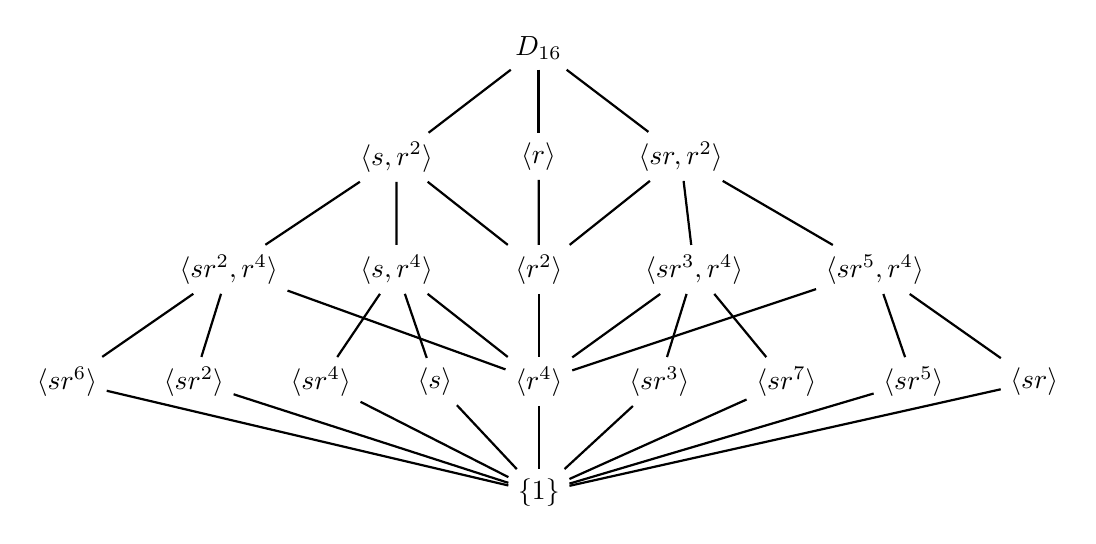
\begin{tikzpicture}[scale=2.5]
        
                \def\d{.8cm}
                \def\h{.6cm}
        
                % Specifies where the x, y coordinate of the tip of
                % the unite vectors in turn
                \tikzset{}
                
                % Scope used to shift the coordinates from the basis
                \begin{scope}[shift={(0, 0, 0)}, rotate=0]
                    \node (D16) at (0, 0) {$D_{16}$};   
                    \node (A1) [below left=\d and \d of D16]
                    {$\langle s, r^2 \rangle$}; 
                    \node (A2) [below= \d of D16] {$\langle r \rangle$}; 
                    \node (A3) [right= \d of A2]
                    {$\langle sr, r^2 \rangle$};  
                    \node (B1) [below left=\d and \d of A1]
                    {$\langle sr^2, r^4 \rangle$}; 
                    \node (B2) [right=\d of B1] {$\langle s, r^4 \rangle$}; 
                    \node (B3) [right=\d of B2]
                    {$\langle r^2 \rangle$};  
                    \node (B4) [right=\d of B3] {$\langle sr^3, r^4 \rangle$}; 
                    \node (B5) [right=\d of B4]
                    {$\langle sr^5, r^4 \rangle$};  
        
                    \node (C1) [below left=\d and \d of B1]
                    {$\langle sr^6 \rangle$}; 
                    \node (C2) [right= \h of C1]
                    {$\langle sr^2 \rangle$}; 
                    \node (C3) [right= \h  of C2]
                    {$\langle sr^4 \rangle$}; 
                    \node (C4) [right= \h of C3]
                    {$\langle s \rangle$}; 
                    \node (C5) [below= \d of B3] {$\langle r^4 \rangle$};
                    \node (C6) [right= \h of C5]
                    {$\langle sr^3 \rangle$}; 
                    \node (C7) [right= \h of C6]
                    {$\langle sr^7 \rangle$};
                    \node (C8) [right= \h of C7]
                    {$\langle sr^5 \rangle$};  
                    \node (C9) [right= \h of C8]
                    {$\langle sr \rangle$};  
                    
                    \node (T1) [below=\d of C5] {$\left\{ 1 \right\}$}; 
                \end{scope}
        
                \begin{scope}[thick]
                    \draw (D16) -- (A1);
                    \draw (D16) -- (A2);
                    \draw (D16) -- (A3);
                    \draw (A1) -- (B1);
                    \draw (A1) -- (B2);
                    \draw (A1) -- (B3);
                    \draw (A3) -- (B5);
                    \draw (A3) -- (B4);
                    \draw (A3) -- (B3);
                    \draw (A2) -- (B3);
                    \draw (B3) -- (C5);
                    \draw (B1) -- (C1);
                    \draw (B1) -- (C2);
                    \draw (B1) -- (C5);
                    \draw (B2) -- (C3);
                    \draw (B2) -- (C4);
                    \draw (B2) -- (C5);
                    \draw (B4) -- (C6);
                    \draw (B4) -- (C7);
                    \draw (B4) -- (C5);
                    \draw (B5) -- (C8);
                    \draw (B5) -- (C9);
                    \draw (B5) -- (C5);
        
                    \foreach\x in {1,..., 9}
                    \draw (C\x) -- (T1);
                \end{scope} 
        
                \end{tikzpicture}
        
                \caption{\label{fig:figure1} Lattice of $D_{16}$.}
            \end{figure} 
                
            $C_{D_{16}}(\{1\}) = D_{16}$, \\
            $C_{D_{16}}(\{r\}) = \langle r \rangle$, \\
            $C_{D_{16}}(\{r^2\}) = \langle r \rangle$, \\
            $C_{D_{16}}(\{r^3\}) = \langle r \rangle$, \\
            $C_{D_{16}}(\{r^4\}) = D_{16}$, \\
            $C_{D_{16}}(\{r^5\}) = \langle r \rangle$, \\
            $C_{D_{16}}(\{r^6\}) = \langle r \rangle$, \\
            $C_{D_{16}}(\{r^7\}) = \langle r \rangle$, \\
            $C_{D_{16}}(\{s\}) = \langle s, r^4 \rangle$, \\
            $C_{D_{16}}(\{sr\}) = \langle r^4, sr^5 \rangle$, \\
            $C_{D_{16}}(\{sr^2\}) = \langle r^4, sr^2 \rangle$, \\
            $C_{D_{16}}(\{sr^3\}) = \langle r^4, sr^2 \rangle$, \\
            $C_{D_{16}}(\{sr^4\}) = \langle s, r^4 \rangle$, \\
            $C_{D_{16}}(\{sr^5\}) = \langle r^4, sr^5 \rangle$, \\
            $C_{D_{16}}(\{sr^6\}) = \langle r^4, sr^2 \rangle$, \\
            $C_{D_{16}}(\{sr^7\}) = \langle r^4, sr^3 \rangle$.  
    \end{enumerate}


    \section*{Exercise 7}
    The center of $D_{16}$ is the set of elements 
    that commute with all others in the group.
    From exercise 1.2.5.6, we know that the only elements
    such that their centralizer is the entire group $D_{16}$
    are $1$ and $r^4$.
    That makes them the only elements in $D_{16}$ to commute
    with the whole group.
    We can also point to exercise 1.2.2.7,
    where we showed $Z(D_{2n}) = \{1, r^n\}$ if $n$ is even.
    So $Z(D_{16}) = \{1, r^4\}$.


    \section*{Exercise 8}
    We know that the normalizers of each group are a subgroup
    of that group,
    so they will feature in its lattice.
    So we will check for each subgroup whether or not it commutes
    set wise with each of the group's subgroups
    to determine the highest subgroup that commutes with it.
    We choose the highest subgroup because the normalizer
    is the set of all elements that have these properties:
    \begin{enumerate}[label=\textbf{\alph*.}]
        \item
            For $S_3$,
            Every subgroup except for the trivial one is maximal,
            and every subgroup is cyclic,
            so every subgroup is contained in its own normalizer.
            That means that for $H \seq S_3$,
            $N_{S_3}(H) = H$ or $S_3$:

            \begin{figure}[H]
                \centering
                % figure is a tikz drawing
                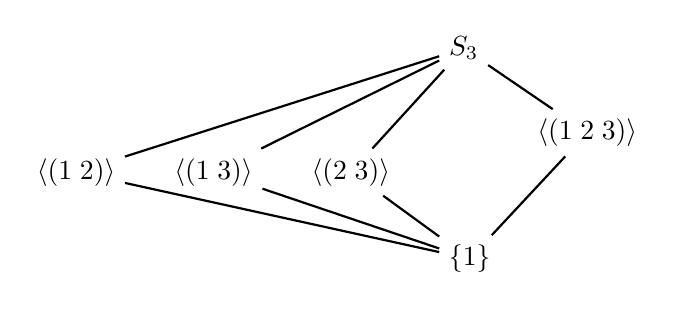
\begin{tikzpicture}[scale=2.5]

                \def\d{.5cm}

                % Specifies where the x, y coordinate of the tip of
                % the unite vectors in turn
                \tikzset{}
                
                % Scope used to shift the coordinates from the basis
                \begin{scope}[shift={(0, 0, 0)}, rotate=0]
                    \node (S3) at (0, 0) {$S_3$};   
                    \node (A1) [below right=\d and \d of S3]
                    {$\langle (1\;2\;3) \rangle$}; 
                    \node (B1) [below left= 2 * \d and \d of S3]
                    {$\langle (2\;3) \rangle$}; 
                    \node (B2) [left= \d of B1]
                    {$\langle (1\;3) \rangle$};  
                    \node (B3) [left= \d of B2]
                    {$\langle (1\;2) \rangle$};  

                    \node (T1) [below right=\d and \d of B1]
                    {$\left\{ 1 \right\}$}; 
                \end{scope}

                \begin{scope}[thick]
                    \draw (S3) -- (A1);
                    \draw (S3) -- (B1);
                    \draw (S3) -- (B2);
                    \draw (S3) -- (B3);
                    \draw (A1) -- (T1);
                    \draw (B1) -- (T1);
                    \draw (B2) -- (T1);
                    \draw (B3) -- (T1);
                \end{scope} 

                \end{tikzpicture}

                \caption{\label{fig:figure1} Lattice of $S_3$.}
            \end{figure} 

            $N_{S_3}(\{1\}) = S_3$, \\
            $N_{S_3}(\langle (1\;2) \rangle) = \langle (1\;2) \rangle$, \\
            $N_{S_3}(\langle (1\;3) \rangle) = \langle (1\;3) \rangle$, \\
            $N_{S_3}(\langle (2\;3) \rangle) = \langle (2\;3) \rangle$, \\
            $N_{S_3}(\langle (1\;2\;3) \rangle) = S_3$, \\
            $N_{S_3}(S_3) = S_3$.

        \item

            For $Q_8$,
            the 3 subgroups generated by imaginary numbers
            are maximal,
            so they either they or the entire group is their own normalizer:
            
            \begin{figure}[H]
                \centering
                % figure is a tikz drawing
                \begin{tikzpicture}[scale=2.5]

                \def\d{.5cm}

                % Specifies where the x, y coordinate of the tip of
                % the unite vectors in turn
                \tikzset{}
                
                % Scope used to shift the coordinates from the basis
                \begin{scope}[shift={(0, 0, 0)}, rotate=0]
                    \node (Q8) at (0, 0) {$Q_8$};   
                    \node (A1) [below left=\d and \d of G1]
                    {$\langle i \rangle$}; 
                    \node (A2) [below= \d of G1] {$\langle j \rangle$}; 
                    \node (A3) [below right=\d and \d of G1]
                    {$\langle k \rangle$};  
                    \node (B3) [below= \d of A2]
                    {$\langle -1 \rangle$};  
                    \node (T1) [below=\d of B3] {$\left\{ 1 \right\}$}; 
                \end{scope}

                \begin{scope}[thick]
                    \draw (Q8) -- (A1);
                    \draw (Q8) -- (A2);
                    \draw (Q8) -- (A3);
                    \draw (A1) -- (B3);
                    \draw (A3) -- (B3);
                    \draw (A2) -- (B3);
                    \draw (B3) -- (T1);
                \end{scope} 

                \end{tikzpicture}
            \caption{\label{fig:figure1} Lattice of $Q_8.$}
            \end{figure} 

            $N_{Q_8}(\{1\}) = Q_8$, \\
            $N_{Q_8}(\langle i \rangle) = Q_8$, \\
            $N_{Q_8}(\langle j \rangle) = Q_8$, \\
            $N_{Q_8}(\langle k \rangle) = Q_8$, \\
            $N_{Q_8}(\langle -1 \rangle) = Q_8$, \\
            $N_{Q_8}(Q_8) = Q_8$.
    \end{enumerate}


    \section*{Exercise 9}
    Referring to exercise 1.2.3.6,
    we know all the subgroups and inclusions
    of $\zbb/48\zbb$ (same applies for $\zbb/16\zbb$ and $\zbb/24\zbb$):
    \begin{enumerate}[label=\textbf{\alph*.}]
        \item
            For $\zbb/16\zbb$:

            \begin{figure}[H]
                \centering
                % figure is a tikz drawing
                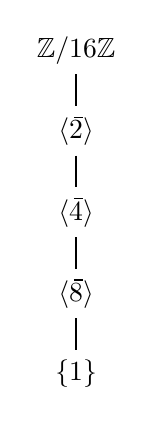
\begin{tikzpicture}[scale=2.5]

                \def\d{.4cm}

                % Specifies where the x, y coordinate of the tip of
                % the unite vectors in turn
                \tikzset{}
                
                % Scope used to shift the coordinates from the basis
                \begin{scope}[shift={(0, 0, 0)}, rotate=0]
                    \node (1) at (0, 0)
                    {$\zbb/16\zbb$}; 
                    \node (2) [below=\d of 1]
                    {$\langle \olsi{2} \rangle$}; 
                    \node (4) [below= \d of 2]
                    {$\langle \olsi{4} \rangle$}; 
                    \node (8) [below= \d of 4]
                    {$\langle \olsi{8} \rangle$};
                    \node (0) [below= \d of 8]
                    {$\{1\}$}; 
                \end{scope}

                \begin{scope}[thick]
                    \draw (1) -- (2);
                    \draw (2) -- (4);
                    \draw (4) -- (8);
                    \draw (8) -- (0);
                \end{scope} 

                \end{tikzpicture}
            \caption{\label{fig:figure1} Lattice of $\zbb/16\zbb$.}
            \end{figure} 
        \item
            For $\zbb/24\zbb$:

            \begin{figure}[H]
                \centering
                % figure is a tikz drawing
                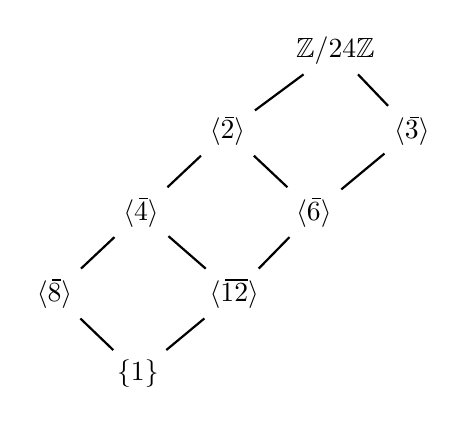
\begin{tikzpicture}[scale=2.5]

                \def\d{.4cm}
                \def\v{0cm}

                % Specifies where the x, y coordinate of the tip of
                % the unite vectors in turn
                \tikzset{}
                
                % Scope used to shift the coordinates from the basis
                \begin{scope}[shift={(0, 0, 0)}, rotate=0]

                    \node (1) at (0, 0) {$\zbb/24\zbb$}; 
                    \node (2) [below left=\d and \d of 1]
                    {$\langle \olsi{2} \rangle$}; 
                    \node (3) [below right=\d and \v of 1]
                    {$\langle \olsi{3} \rangle$}; 
                    \node (4) [below left=\d and \d of 2]
                    {$\langle \olsi{4} \rangle$}; 
                    \node (6) [below right=\d and \d of 2]
                    {$\langle \olsi{6} \rangle$}; 
                    \node (8) [below left=\d and \d of 4]
                    {$\langle \olsi{8} \rangle$}; 
                    \node (12) [below right=\d and \d of 4]
                    {$\langle \olsi{12} \rangle$}; 
                    \node (0) [below left=\d and \d of 12]
                    {$\{1\}$}; 
                \end{scope}

                \begin{scope}[thick]
                    \draw (1) -- (2);
                    \draw (1) -- (3);
                    \draw (2) -- (4);
                    \draw (2) -- (6);
                    \draw (4) -- (8);
                    \draw (4) -- (12);
                    \draw (3) -- (6);
                    \draw (6) -- (12);
                    \draw (8) -- (0);
                    \draw (12) -- (0);
                \end{scope} 

                \end{tikzpicture}
            \caption{\label{fig:figure1} Lattice of $\zbb/24\zbb$.}
            \end{figure} 
        \item
            For $\zbb/48\zbb$:

            \begin{figure}[H]
                \centering
                % figure is a tikz drawing
                \begin{tikzpicture}[scale=2.5]

                \def\d{.4cm}
                \def\v{0cm}

                % Specifies where the x, y coordinate of the tip of
                % the unite vectors in turn
                \tikzset{}
                
                % Scope used to shift the coordinates from the basis
                \begin{scope}[shift={(0, 0, 0)}, rotate=0]

                    \node (1) at (0, 0) {$\zbb/48\zbb$}; 
                    \node (2) [below left=\d and \d of 1]
                    {$\langle \olsi{2} \rangle$}; 
                    \node (3) [below right=\d and \v of 1]
                    {$\langle \olsi{3} \rangle$}; 
                    \node (4) [below left=\d and \d of 2]
                    {$\langle \olsi{4} \rangle$}; 
                    \node (6) [below right=\d and \d of 2]
                    {$\langle \olsi{6} \rangle$}; 
                    \node (8) [below left=\d and \d of 4]
                    {$\langle \olsi{8} \rangle$}; 
                    \node (12) [below right=\d and \d of 4]
                    {$\langle \olsi{12} \rangle$}; 
                    \node (16) [below left=\d and \d of 8]
                    {$\langle \olsi{16} \rangle$}; 
                    \node (24) [below right=\d and \d of 8]
                    {$\langle \olsi{24} \rangle$};  
                    \node (0) [below left=\d and \d of 24]
                    {$\{1\}$}; 
                \end{scope}

                \begin{scope}[thick]
                    \draw (1) -- (2);
                    \draw (1) -- (3);
                    \draw (2) -- (4);
                    \draw (2) -- (6);
                    \draw (4) -- (8);
                    \draw (4) -- (12);
                    \draw (8) -- (16);
                    \draw (8) -- (24);
                    \draw (16) -- (0);
                    \draw (3) -- (6);
                    \draw (6) -- (12);
                    \draw (12) -- (24);
                    \draw (24) -- (0);
                \end{scope} 

                \end{tikzpicture}
            \caption{\label{fig:figure1} Lattice of $\zbb/48\zbb$.}
            \end{figure} 
    \end{enumerate}


    \section*{Exercise 10 $***$}
    Proof that if $|G| = 4$, 
    then $G \cong Z_4$ (cyclic group) or $G \cong V_4$ (Klein 4-group): \\
    We know from our proof in exercise 1.1.1.36 that a group
    of order 4 where none of the elements have order 4
    is unique and has the following table:
    \begin{figure}[H]
        \centering

        \[\vbox{\tabskip0.5em\offinterlineskip
        \halign{\strut$#$\hfil\ \tabskip1em\vrule&&$#$\hfil\cr
        ~   & 1   & a   & b & c \cr
        \noalign{\hrule}\vrule height 12pt width 0pt
        1   & 1 & a & b & c \cr 
        a   & a & 1 & c & b \cr 
        b   & b & c & 1 & a \cr 
        c   & c & b & a & 1 \cr
        }}\]

        \caption{\label{fig:figure1} The table of the described group.}
    \end{figure}
    
    This is obviously the group table of the Klein 4-group,
    so every group of order 4 that doesn't have
    an element with order 4 is unique and isomorphic to $V_4$. \\
    To add to the prood, if $|G| = 4$ and there exists
    an element $x \in G$ with order 4 as well,
    then by exercise 1.1.1.32, since $|x| = 4$,
    $1, x, x^2, x^3$ are all unique elements.
    Since $G$ is closed under multiplication,
    all 4 elements are in $G$.
    And since $G = 4$, then $G = \{1, x, x^2, x^3\}$.
    So $G = Z_4$.
    So any group of order 4 where one element has order 4 as well
    must be isomorphic to $Z_4$.


    \section*{Exercise 11 $***$}
    Let
    \[ QD_{16} = \langle \sigma, \tau \mid \sigma^8 = \tau^2 = 1,
    \sigma\tau = \tau\sigma^3 \rangle \] 
    Be a group of order 16
    (called the \textit{Quasidihedral} or \textit{Semidihedral
    Group of order 16}).
    This group has 3 subgroups of order 8,
    which are
    \[ \langle \tau, \sigma^2 \rangle \cong D_8, \qquad
    \langle \sigma \rangle \cong Z_8, \qquad
    \langle \sigma^2, \tau\sigma \rangle \cong Q_8 \]
    Every proper subgroup of $QD_{16}$ is contained inside one of those
    3 subgroups.
    To complete the given lattice of $QD_{16}$ by filling in the missing
    subgroups using at most two generators,
    we can use the lattices of $D_8$, $Z_8$ and $Q_8$
    in order to help us,
    since isomorphic groups have the same lattices. \\
    According to exercise 1.1.5.3,
    $Q_8$ is generated by $i$ and $j$,
    so $\langle i, j \rangle \cong \langle \sigma^2, \tau\sigma \rangle$.
    We know that $Q_8$ has 3 maximal subgroups,
    $\langle i \rangle$, $\langle j \rangle$, and $\langle k \rangle$,
    all of which are cyclic.
    This means that in $QD_{16}$,
    $\langle \sigma^2, \tau\sigma \rangle$
    will have 3 subgroups,
    $\langle \sigma^2 \rangle$,
    $\langle \tau\sigma \rangle$
    and 
    $\langle \sigma^2\tau\sigma \rangle$
    (since $ij = k$).
    The leftmost subgroup is supposed to be $\langle \sigma^2 \rangle$
    because it's contained inside $\langle \sigma \rangle$,
    which is cyclic and only contains cyclic subgroups generated
    by a power of $\sigma$.
    The order of the other two doesn't matter. \\
    Now if we look at the lattice of $D_8$,
    we note that it also has 3 maximal subgroups,
    which are $\langle r \rangle$,
    $\langle s, r^2 \rangle$, 
    and $\langle rs, r^2 \rangle$.
    We know that
    $D_8 = \langle r, s \rangle \cong \langle \sigma^2, \tau \rangle$,
    so if we map $r$ to $\sigma^2$ and $s$ to $\tau$,
    we see that in the $QD_{16}$ lattice,
    $\langle \sigma^2, \tau \rangle$
    already contains $\langle \sigma^2\rangle$, or $\langle r \rangle$,
    and $\langle \sigma^4, \tau \rangle$, or $\langle r^2, s \rangle$.
    This leaves $\langle rs, r^2  \rangle$,
    which in this case is the leftmost subgroup
    $\langle \sigma^2\tau, \sigma^4 \rangle$. \\
    Now in $D_8$,
    the subgroup $\langle r^2, s  \rangle$
    also contains 3 subgroups,
    which are $\langle r^2 \rangle$,
    $\langle s \rangle$,
    and $\langle r^2s \rangle$,
    which correspond to
    $\langle \sigma^4 \rangle$,
    $\langle \tau \rangle$,
    and $\langle \sigma^4\tau \rangle$.
    These will be the subgroups of
    $\langle \sigma^4, \tau \rangle$ in the lattice.
    The first two of the subgroups already exist,
    so we add the third. \\
    Also in $D_8$ is the subgroup $\langle rs, r^2  \rangle$
    also contains 3 subgroups,
    which are $\langle r^2 \rangle$,
    $\langle rs \rangle$,
    and $\langle r^3s \rangle$,
    which correspond to
    $\langle \sigma^4 \rangle$,
    $\langle \sigma^2\tau \rangle$,
    and $\langle \sigma^6\tau \rangle$.
    These will be the subgroups of
    $\langle \sigma^2\tau, \sigma^4 \rangle$ in the lattice.
    The first and third the subgroups already exist.
    This is because, for the third subgroup,
    $\sigma^6\tau = \sigma^{5}\sigma\tau = \sigma^5\tau\sigma^3 = \dots
    = \tau\sigma^{18} = \tau\sigma^{16}\sigma^2
    = \tau(\sigma^{8})^2\sigma^2 = \tau\sigma^2$.
    So we add the second subgroup $\langle \sigma^2\tau \rangle$
    to the lattice.

    \begin{figure}[H]
        \centering
        % figure is a tikz drawing
        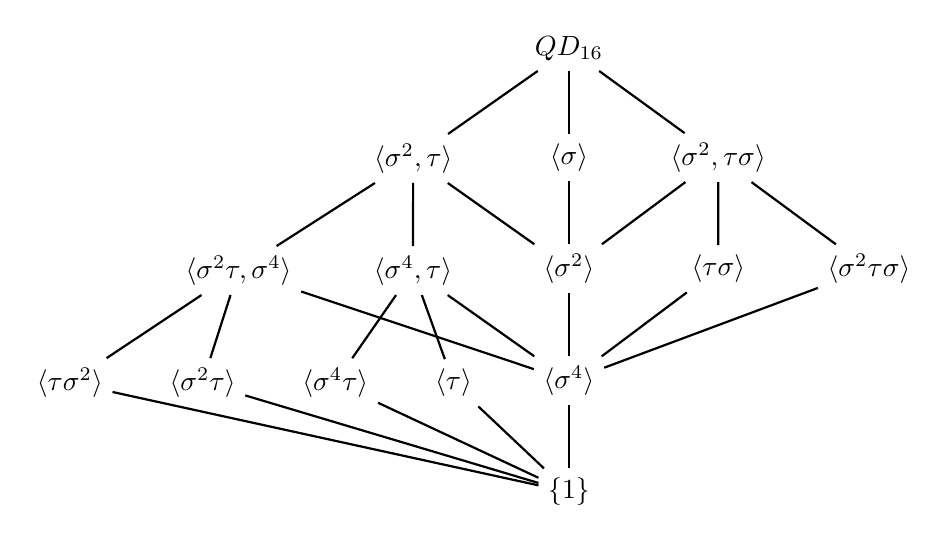
\begin{tikzpicture}[scale=2.5]

        \def\d{.8cm}
        \def\h{.6cm}

        % Specifies where the x, y coordinate of the tip of
        % the unite vectors in turn
        \tikzset{}
        
        % Scope used to shift the coordinates from the basis
        \begin{scope}[shift={(0, 0, 0)}, rotate=0]
            \node (D16) at (0, 0) {$QD_{16}$};   
            \node (A1) [below left=\d and \d of D16]
            {$\langle \sigma^2, \tau \rangle$}; 
            \node (A2) [below= \d of D16] {$\langle \sigma \rangle$}; 
            \node (A3) [right= \d of A2]
            {$\langle \sigma^2, \tau\sigma \rangle$};  
            \node (B1) [below left=\d and \d of A1]
            {{$\langle \sigma^2\tau, \sigma^4 \rangle$}}; 
            \node (B2) [right=\d of B1] {$\langle \sigma^4, \tau \rangle$}; 
            \node (B3) [below=\d of A2]
            {{$\langle \sigma^2 \rangle$}};  
            \node (B4) [below=\d of A3]
            {{$\langle \tau\sigma \rangle$}}; 
            \node (B5) [right=\d of B4]
            {{$\langle \sigma^2\tau\sigma \rangle$}};  

            \node (C1) [below left=\d and \d of B1]
            {$\langle \tau\sigma^2 \rangle$}; 
            \node (C2) [right= \h of C1]
            {{$\langle \sigma^2\tau \rangle$}}; 
            \node (C3) [right= \h  of C2]
            {{$\langle \sigma^4\tau \rangle$}}; 
            \node (C4) [right= \h of C3]
            {$\langle \tau \rangle$}; 
            \node (C5) [below= \d of B3] {$\langle \sigma^4 \rangle$};

            
            \node (T1) [below=\d of C5] {$\left\{ 1 \right\}$}; 
        \end{scope}

        \begin{scope}[thick]
            \draw (D16) -- (A1);
            \draw (D16) -- (A2);
            \draw (D16) -- (A3);
            \draw (A1) -- (B1);
            \draw (A1) -- (B2);
            \draw (A1) -- (B3);
            \draw (A3) -- (B5);
            \draw (A3) -- (B4);
            \draw (A3) -- (B3);
            \draw (A2) -- (B3);
            \draw (B3) -- (C5);
            \draw (B1) -- (C1);
            \draw (B1) -- (C2);
            \draw (B1) -- (C5);
            \draw (B2) -- (C3);
            \draw (B2) -- (C4);
            \draw (B2) -- (C5);
            \draw (B4) -- (C5);
            \draw (B5) -- (C5);

            \foreach\x in {1,..., 5}
            \draw (C\x) -- (T1);
        \end{scope} 

        \end{tikzpicture}

        \caption{\label{fig:figure1} Lattice of $QD_{16}$.}
    \end{figure} 


    \section*{Exercise 12}
    Consider the group 
    \[A = Z_2 \times Z_4 = \langle a, b \mid a^2 = b^4 = 1, ab = ba \rangle\]
    where $A$ has order $8$ and three subgroups of order $4$:
    \[\langle a, b^2 \rangle \cong V_4 
    \qquad \langle b \rangle \cong Z_4
    \qquad \langle ab \rangle \cong Z_4 \]
    and where every other proper subrgoup is contained in of these three.
    We need to draw $A$'s lattice 
    with each subgroup represented using at most $2$ generators. \\
    We know $Z_4$ has a subgroup for each positive integer that divides $4$.
    So both $Z_2$ and $Z_1 = {1}$ are subgroups of $Z_4$. \\
    We know that $Z_4 \cong \langle b \rangle$,
    so $Z_2 \cong \langle b^2 \rangle$. \\ 
    Likewise, we know that $Z_4 \cong \langle ab \rangle$,
    so $Z_2 \cong \langle a^2b^2 \rangle = \langle b^2 \rangle$. \\ 
    Moreover, we know that if $V_4$ is the Klein 4-group,
    then it has $3$ subgroups of order $2$.
    We know that if $V_4$ is generated by $a$ and $b$
    (where $ab = c$),
    then those subgroups are
    \[ \langle a \rangle
    \qquad \langle b \rangle 
    \qquad \langle ab \rangle \]
    which, if $V_4 \cong \langle a, b^2 \rangle$,
    means that those subgroups are
    \[ \langle a \rangle
    \qquad \langle b^2 \rangle 
    \qquad \langle ab^2 \rangle \]
    So, bringing it all together,
    we have the following lattice.
    \begin{figure}[H]
        \centering
        % figure is a tikz drawing
        \begin{tikzpicture}[scale=2.5]

        \def\d{.8cm}

        % Specifies where the x, y coordinate of the tip of
        % the unite vectors in turn
        \tikzset{}
        
        % Scope used to shift the coordinates from the basis
        \begin{scope}[shift={(0, 0, 0)}, rotate=0]
            \node (Q8) at (0, 0) {$A$};   
            \node (A1) [below left=\d and \d of G1]
            {$\langle a, b^2 \rangle$}; 
            \node (A2) [below= \d of G1] {$\langle b \rangle$}; 
            \node (A3) [below right=\d and \d of G1]
            {$\langle ab \rangle$};  
            \node (B1) [below left=\d and \d of A1]
            {$\langle a \rangle$}; 
            \node (B2) [below= \d of A1] {$\langle ab^2 \rangle$}; 
            \node (B3) [below=\d of A2]
            {$\langle b^2 \rangle$}; 
            \node (T1) [below=\d of B2] {$\left\{ 1 \right\}$}; 
        \end{scope}

        \begin{scope}[thick]
            \foreach\x in {1,..., 3}
            \draw (Q8) -- (A\x);
            \draw (A1) -- (B1);
            \draw (A1) -- (B2);
            \draw (A1) -- (B3);
            \draw (A3) -- (B3);
            \draw (A2) -- (B3);
            \foreach\x in {1,..., 3}
            \draw (B\x) -- (T1);
        \end{scope} 

        \end{tikzpicture}

        \caption{\label{fig:figure1} Lattice of $A.$}
    \end{figure} 


    \section*{Exercise 13}
    Consider the group 
    \[G = Z_2 \times Z_8 = \langle x, y \mid x^2 = y^8 = 1, xy = yx \rangle\]
    where $A$ has order $16$ and three subgroups of order $8$:
    \[\langle x, y^2 \rangle \cong Z_2 \times Z_4 
    \qquad \langle y \rangle \cong Z_8
    \qquad \langle xy \rangle \cong Z_8 \]
    and where every other proper subgroup is contained in one of them.
    We need to draw the lattice of subgroups of $G$
    with no more than $2$ generators each. \\
    First, according to exercise 1.2.4.12,
    we know the lattice of a subgroup
    \[ Z_2 \times Z_4 = \langle a, b \mid a^2 = b^4 = 1, ab = ba \rangle \]
    We already know that $\langle x, y^2 \rangle \cong Z_2 \times Z_4$,
    and since $x$ and $y^2$ fufill all relations of $a$ and $b$,
    we can replace $a$ and $b$
    in the lattice of $Z_2 \times Z_4$,
    generating the following lattice.
    
    \begin{figure}[H]
        \centering
        % figure is a tikz drawing
        \begin{tikzpicture}[scale=2.5]

        \def\d{.8cm}

        % Specifies where the x, y coordinate of the tip of
        % the unite vectors in turn
        \tikzset{}
        
        % Scope used to shift the coordinates from the basis
        \begin{scope}[shift={(0, 0, 0)}, rotate=0]
            \node (Q8) at (0, 0) {$\langle x, y^2 \rangle$};   
            \node (A1) [below left=\d and \d of G1]
            {$\langle x, y^4 \rangle$}; 
            \node (A2) [below= \d of G1] {$\langle xy^2 \rangle$}; 
            \node (A3) [below right=\d and \d of G1]
            {$\langle y^2 \rangle$};  
            \node (B1) [below left=\d and \d of A1]
            {$\langle x \rangle$}; 
            \node (B2) [below= \d of A1] {$\langle xy^4 \rangle$}; 
            \node (B3) [below=\d of A2]
            {$\langle y^4 \rangle$}; 
            \node (T1) [below=\d of B2] {$\left\{ 1 \right\}$}; 
        \end{scope}

        \begin{scope}[thick]
            \foreach\x in {1,..., 3}
            \draw (Q8) -- (A\x);
            \draw (A1) -- (B1);
            \draw (A1) -- (B2);
            \draw (A1) -- (B3);
            \draw (A3) -- (B3);
            \draw (A2) -- (B3);
            \foreach\x in {1,..., 3}
            \draw (B\x) -- (T1);
        \end{scope} 

        \end{tikzpicture}

        \caption{\label{fig:figure1} Lattice of $\langle x, y^2 \rangle.$}
    \end{figure} 

    Moreover, we know that 
    $\langle y \rangle \cong \langle xy \rangle \cong Z_8$.
    So we know that for each positive integer divisor of $8$,
    we will have a subgroup. \\
    So for $\langle y \rangle$ the proper subgroups are
    \[ \langle y^2 \rangle
    \qquad \langle y^4 \rangle
    \qquad \{1\}\]
    And for $\langle xy \rangle$,
    the proper subrgoups are
    \[ \langle x^2y^2 \rangle = \langle y^2 \rangle
    \qquad \langle x^4y^4 \rangle = \langle y^4 \rangle
    \qquad \{1\}\]
    With all that, we can draw this lattice.
    
    \begin{figure}[H]
        \centering
        % figure is a tikz drawing
        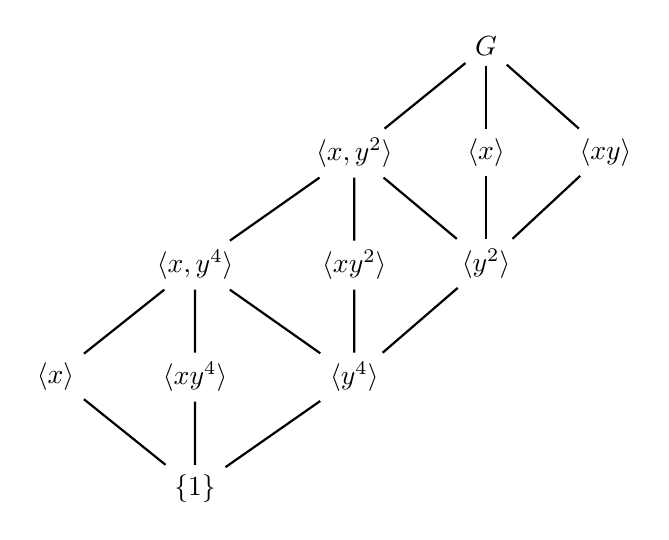
\begin{tikzpicture}[scale=2.5]

        \def\d{.8cm}

        % Specifies where the x, y coordinate of the tip of
        % the unite vectors in turn
        \tikzset{}
        
        % Scope used to shift the coordinates from the basis
        \begin{scope}[shift={(0, 0, 0)}, rotate=0]

            \node (Q1) at (0, 0) {$G$};
            \node (Z1) [below left=\d and \d of Q1]
            {$\langle x, y^2 \rangle$};
            \node (Z2) [below=\d of Q1]
            {$\langle x \rangle$};
            \node (Z3) [below right=\d and \d of Q1] 
            {$\langle xy \rangle$};
            \node (A1) [below left=\d and \d of Z1]
            {$\langle x, y^4 \rangle$};         
            \node (A2) [below= \d of Z1] {$\langle xy^2 \rangle$}; 
            \node (A3) [below=\d of Z2]
            {$\langle y^2 \rangle$};  
            \node (B1) [below left=\d and \d of A1]
            {$\langle x \rangle$}; 
            \node (B2) [below= \d of A1] {$\langle xy^4 \rangle$}; 
            \node (B3) [below=\d of A2]
            {$\langle y^4 \rangle$}; 
            \node (T1) [below=\d of B2] {$\left\{ 1 \right\}$}; 
        \end{scope}

        \begin{scope}[thick]
            \foreach\x in {1,..., 3}
            \draw (Q1) -- (Z\x);
            \foreach\x in {1,..., 3}
            \draw (Z1) -- (A\x);

            \draw (Z2) -- (A3);
            \draw (Z3) -- (A3);

            \draw (A1) -- (B1);
            \draw (A1) -- (B2);
            \draw (A1) -- (B3);
            \draw (A3) -- (B3);
            \draw (A2) -- (B3);

            \foreach\x in {1,..., 3}
            \draw (B\x) -- (T1);
        \end{scope} 

        \end{tikzpicture}

        \caption{\label{fig:figure1} Lattice of $G.$}
    \end{figure} 


    \section*{Exercise 14}
    Suppose that
    \[ M = \langle u, v \mid u^2 = v^8 = 1, vu = uv^5 \rangle \] 
    has order $16$
    (the group is sometimes called the \textit{modular group of order $16$}).
    We know that there are three subgroups of order $8$
    \[ \langle u, v^2 \rangle
    \qquad \langle v \rangle 
    \qquad \langle uv \rangle \]
    and that every other proper subgroup of $M$ is contained
    in one of them. \\
    First we show that $\langle u, v^2 \rangle \cong Z_2 \times Z_4$.
    We know from exercise 1.2.5.12
    the presentation of $Z_2 \times Z_4$,
    and we note that if we map $u$ to $a$, and $v^2$ to $b$,
    then we've mapped all generators in the former
    to all of the generators in the latter.
    Moreover, the relation $u^2 = (v^2)^4 = v^8 = 1$ is satisfied.
    So we have a homomorphism.
    Furthermore, by our construction,
    the mapping is surjective
    (since the values we mapped to, $a$ and $b$, generate $Z_2 \times Z_4$,
    we can then map to any other element in the group),
    and $|\langle u, v^2 \rangle| = |Z_2 \times Z_4| = 8$,
    making the mapping a bijection.
    So $\langle u, v^2 \rangle \cong Z_2 \times Z_4$. \\
    Likewise, we have 
    \[\langle v \rangle = \{v, v^2, v^3, v^4, v^5, v^6, v^7, 1\} \]
    and
    \[\langle uv \rangle = \{uv, v^2, uv^3, v^4, uv^5, v^6, uv^7, 1\} \]
    which tells us that the both groups are isomorphic to $Z_8$ 
    as all cyclic subgroups of the same order are isomorphic. \\ 
    Since these groups are respectively isomorphic,
    we can place $u$ and $v$ in the lattice of $G$
    from exercise 1.2.5.13, which has the same three subgroups.

    \begin{figure}[H]
        \centering
        % figure is a tikz drawing
        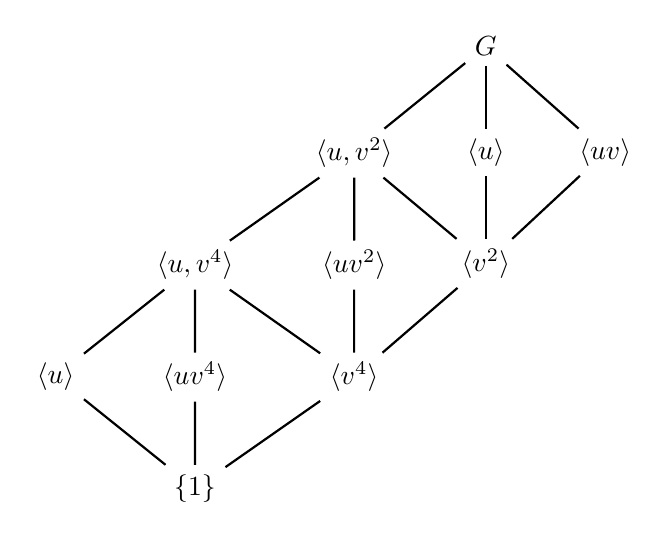
\begin{tikzpicture}[scale=2.5]

        \def\d{.8cm}

        % Specifies where the x, y coordinate of the tip of
        % the unite vectors in turn
        \tikzset{}
        
        % Scope used to shift the coordinates from the basis
        \begin{scope}[shift={(0, 0, 0)}, rotate=0]

            \node (Q1) at (0, 0) {$G$};
            \node (Z1) [below left=\d and \d of Q1]
            {$\langle u, v^2 \rangle$};
            \node (Z2) [below=\d of Q1]
            {$\langle u \rangle$};
            \node (Z3) [below right=\d and \d of Q1] 
            {$\langle uv \rangle$};
            \node (A1) [below left=\d and \d of Z1]
            {$\langle u, v^4 \rangle$};         
            \node (A2) [below= \d of Z1] {$\langle uv^2 \rangle$}; 
            \node (A3) [below=\d of Z2]
            {$\langle v^2 \rangle$};  
            \node (B1) [below left=\d and \d of A1]
            {$\langle u \rangle$}; 
            \node (B2) [below= \d of A1] {$\langle uv^4 \rangle$}; 
            \node (B3) [below=\d of A2]
            {$\langle v^4 \rangle$}; 
            \node (T1) [below=\d of B2] {$\left\{ 1 \right\}$}; 
        \end{scope}

        \begin{scope}[thick]
            \foreach\x in {1,..., 3}
            \draw (Q1) -- (Z\x);
            \foreach\x in {1,..., 3}
            \draw (Z1) -- (A\x);

            \draw (Z2) -- (A3);
            \draw (Z3) -- (A3);

            \draw (A1) -- (B1);
            \draw (A1) -- (B2);
            \draw (A1) -- (B3);
            \draw (A3) -- (B3);
            \draw (A2) -- (B3);

            \foreach\x in {1,..., 3}
            \draw (B\x) -- (T1);
        \end{scope} 

        \end{tikzpicture}

        \caption{\label{fig:figure1} Lattice of $M.$}
    \end{figure} 

    So in conclusion, $G = Z_2 \times Z_8$ has the same lattice as
    as $M$,
    since both have the same shape
    (more formally, we can map the subgroups of $G$ to those of $M$,
    in such a way as to preserve all subgroup relationships). \\
    Proof that $M \ncong G$:\\
    We know that two groups need not be isomorphic
    in order to have the same lattice.
    Knowing that, we can show that $M \ncong G$
    since $G$ is abelian
    ($xy = yx$ implies all other elements in the group generated by $x$
    and $y$ commute),
    and $M$ is not ($vu = uv^5$ and $v \neq v^5$).


    \section*{Exercise 15}
    We know that $D_16$ has three subgroups of order $8$:
    \[ \langle s, r^2 \rangle 
    \qquad  \langle r \rangle
    \qquad \langle sr, r^2 \rangle \]
    We know that $\langle r \rangle$ is cyclic,
    and that $|\langle r \rangle| = 8$,
    so $\langle r \rangle \cong Z_8$. \\
    Next, we note that
    \[ D_8 = \langle s, r \mid s^2 = r^4 = 1, rs = sr^{-1} \rangle \]
    We notice that if we map the generators $r$ and $s$
    to those of $\langle s, r^2 \rangle$ such that $s$ is mapped to $s$
    and $r$ to $r^2$,
    all the relations are preserved.
    This makes the two groups homomorphic.
    Next we note that the mapping is surjective by construction
    (as $r^2$ and $s$ generate the group by definition),
    and that the two subgroups have the same order $8$.
    So the the mapping is bijective,
    and $\langle sr, r^2 \rangle \cong D_8$. \\
    Likewise, if we map the generators $r$ and $s$ of $D_8$
    to those of $\langle sr, r^2 \rangle$ such that $s$ is mapped to $sr$
    and $r$ to $r^2$,
    all the relations are preserved.
    This makes the two groups homomorphic.
    Next we note that the mapping is surjective by construction
    (as $r^2$ and $sr$ generate the group by definition),
    and that the two subgroups have the same order $8$.
    So the the mapping is bijective,
    and $\langle sr, r^2 \rangle \cong D_8$. \\


    \section*{Exercise 16 $***$}
    Proof that all elements of order $2$
    of the Quasidihedral group of order $16$
    (from exercise 1.2.5.11)
    are contained in the subgroup $\langle \tau, \sigma^2 \rangle$
    using the lattice of $QD_{16}$. \\
    We know that every element of order $2$
    generates a cyclic group of order $2$,
    which is trivially a subgroup of $QD_{16}$.
    The only cyclic groups present in the lattice
    that aren't subgroups (below) $\langle \tau, \sigma^2 \rangle$ are
    \[ \langle \sigma \rangle 
    \qquad \text{and} 
    \qquad \tau\sigma \]
    neither of which has order $2$.
    So we can confidently say that all cyclic groups of order $2$
    are subgroups of $\langle \tau, \sigma^2 \rangle$,
    and by extension, that their generators,
    which form all the elements of order $2$ in $QD_{16}$,
    belong to $\langle \tau, \sigma^2 \rangle$.


    \section*{Exercise 17 $***$}
    Proof that the set $\{x \in M \mid x^2 = 1\}$ 
    ($M$ is the modular group of order $16$ from exercise 1.2.5.14),
    is a subgroup of $M$ isomorphic to the Klein 4-group,
    using the lattice of $M$. \\ 
    Suppose we call the set $H$. \\
    We know that only the identity $1$ has order $1$,
    so all other elements of the set must have order $2$.
    Elements of order $2$ generate each a cyclic group of order $2$
    that is trivially a subgroup of $M$.
    These subgroups will necessarily show up in the lattice. \\
    Indeed we have three:
    \[ \langle v^4 \rangle 
    \qquad \langle u \rangle 
    \qquad \langle uv^4 \rangle  \]
    This means that $H = \{ 1, u, v^4, uv^4 \}$. \\
    This is clearly a subgroup of $M$ as it is non-empty,
    all elements are their own inverses (as tehy have order $2$),
    and the mutliplication of any two elements that aren't the identity
    gives the third non-identity element. \\
    Furthermore, we know that this group is isomorphic to $V_4$.
    If we look at the lattice of $M$,
    we notice that all three of the above mentioned cyclic groups
    belong to $\langle u, v^4 \rangle$,
    which we know has order $4$
    (as it is sandwiched between groups of order $8$ and $2$,
    and $4$ is the only other number that divides $8$ besides $1$). \\
    Since all three generators as well as the identity belong to it,
    that must mean that $\langle u, v^4 \rangle = H$.
    All groups of order $4$ are isomorphic to $Z_4$ or $V_4$,
    and since $\langle u, v^4 \rangle$ is not cyclic,
    it must be isomorphic to $V_4$.


    \section*{Exercise 18 $***$}
    Using the lattice of subgroups of $QD_{16}$
    from exercise 1.2.5.11,
    we will find the centralizers of all of the group's elements. \\
    First we note that all centralizers are subgroups of $QD_{16}$
    and must therefore appear in the lattice. \\
    We also note that
    \[ QD_{16} = \langle \sigma, \tau \mid \sigma^8 = \tau^2 = 1,
    \sigma\tau = \tau\sigma^3 \rangle \]
    All other powers of $\sigma$ commute with any power of $\sigma$,
    but not $\tau$.
    This means that the centralizer of each power of $\sigma$ can only be
    the cyclic group $\langle \sigma \rangle$,
    as it is the only subgroup containing all powers of $\sigma$
    but not $\tau$
    (since there are $8$ powers of $\sigma$,
    and $8$ is the order of the largest proper subgroup in the lattice). \\
    The elements $1$ and $\sigma^4$ however,
    commute with all other elements,
    so their centralizer is $QD_{16}$. \\
    We also have 
    \[ \tau\sigma^4 
    = \tau\sigma^3\sigma
    = \sigma\tau\sigma 
    = \sigma\sigma^3\tau
    = \sigma^4\tau \] 
    Since $\sigma^4, \tau \in C_{QD_{16}}(\tau)$,
    then $\langle \tau, \sigma^4 \rangle \leqslant C_{QD_{16}}(\tau)$
    (this is because $\langle \tau, \sigma^4 \rangle$
    is the smallest subgroup containing both elements). \\
    Reffering to the lattice,
    that means that $C_{QD_{16}}(\tau)$
    is $\langle \tau, \sigma^4 \rangle$,
    or $\langle \tau, \sigma^2 \rangle$,
    or $QD_{16}$.
    Since $\sigma^2$ does not commute with $\tau$,
    it is not part of its centralizer,
    which means that  $C_{QD_{16}}(\tau)$ must instead be equal to
    $\langle \tau, \sigma^4 \rangle$. \\
    For the rest of elements of the form $\tau\sigma^i$,w
    we can apply the same argument, and get that: \\\
    \[ C_{QD_{16}}(\tau\sigma^4) 
    = C_{QD_{16}}(\tau) 
    = \langle \tau, \sigma^4 \rangle \]
    \[ C_{QD_{16}}(\tau\sigma^5) 
    = C_{QD_{16}}(\tau\sigma^1) 
    = \langle \tau\sigma \rangle \]
    \[ C_{QD_{16}}(\tau\sigma^6) 
    = C_{QD_{16}}(\tau\sigma^2) 
    = \langle \sigma^2\tau, \sigma^4 \rangle \]
    \[ C_{QD_{16}}(\tau\sigma^7) 
    = C_{QD_{16}}(\tau\sigma^3) 
    = \langle \tau\sigma^7 \rangle
    =  \langle \sigma^2\tau\sigma \rangle \]
    The process is time consuming but straighforward;
    we find elements that commute,
    and eliminate subgroups from the lattice until we are left with one.



    \section*{Exercise 19}
    Using the lattice of $D_{16}$ to find the normalizer 
    $N_{D_{16}}(\langle s, r^4 \rangle)$. \\
    First, we know that 
    \[ \langle s, r^4 \rangle = \{ 1, s, sr^4, r^4 \} \]
    Notice that $s$ obviously belongs to the normalizer,
    as $s = s^{-1}$,
    so $s\langle s, r^4 \rangle s^{-1} = s\langle s, r^4 \rangle s$. \\
    This gives us $s1s = 1ss = 1$, 
    $sss = 1s = s$,  
    $ssr^4s = r^4s = sr^4$,
    and $sr^4s = ssr^4 = r^4$. \\
    The same applies for $r^2$, as $(r^2)^{-1} = r^6$.
    We have $s\langle s, r^4 \rangle s^{-1} = s\langle s, r^4 \rangle s$,
    which in turn gives us
    $r^21r^6 = r^8 = 1$,    
    $r^2sr^6 = sr^{-2}r^6 = sr^4$,
    $r^2sr^4r^6 = sr^{-2}r^4r^6 = sr^8 = s$,
    $r^2r^4r^6 = r^12 = r^4$.
    So $r^2$ and $s$ both belong to the normalizer. \\
    Since the normalizer is a subgroup,
    it must be part of the lattice,
    and we know that 
    $\langle s, r^2 \rangle \leqslant N_{D_{16}}(\langle s, r^4 \rangle)$
    (as $\langle s, r^2 \rangle$ is the smallest subgroup
    containing both elements).
    That means that $N_{D_{16}}(\langle s, r^4 \rangle)$ is either
    $\langle s, r^2 \rangle$ or $D_{16}$.
    It can't be the latter as $r$ is not part of the normalizer,
    (which can be checked).
    So $N_{D_{16}}(\langle s, r^4 \rangle) = \langle s, r^2 \rangle$.


    \section*{Exercise 20}    
    Using the lattice of $QD_{16}$ (from exercise 1.2.5.11)
    to find the normalizers
    $N_{QD_{16}}(\langle \tau\sigma \rangle)$
    and $N_{QD_{16}}(\langle \tau, \sigma^4 \rangle)$. \\
    \begin{enumerate}[label=\textbf{\alph*.}]
        \item
            Similarly to exercise 1.2.5.19,
            we start by testing that the values $\sigma^2$ belongs in the
            normalizer. Same for $\tau\sigma$. \\
            When we do that, we will learn that
            $\tau\sigma$ and $\sigma^2$ belong to the normalizer.
            So as the normalizer is a group,
            and since $\langle \tau\sigma, \sigma^2 \rangle$ is the
            smallest group containing them,
            $\langle \tau\sigma, \sigma^2 \rangle \leqslant 
            N_{QD_{16}}(\langle \tau\sigma \rangle)$. \\
            So the normalizer can be $\langle \tau\sigma, \sigma^2 \rangle$,
            or $QD_{16}$,
            however, as $\tau$ does not belong to the normalizer
            (which may be tested),
            it can't be $QD_{16}$,
            so it must then be that 
            $ N_{QD_{16}}(\langle \tau\sigma \rangle)
            = \langle \tau\sigma, \sigma^2 \rangle$.
        \item
            For $N_{QD_{16}}(\langle \tau, \sigma^4 \rangle)$,
            we can repeat the same process,
            this time with $\sigma^2$ and $\tau$.
            We will realize that both belong to the normalizer,
            so that
            $\langle \sigma^2, \tau \rangle
            \leqslant N_{QD_{16}}(\langle \tau, \sigma^4 \rangle)$.
            So the normalizer can be $\langle \sigma^2, \tau \rangle$,
            or $QD_{16}$.
            However, since $\sigma$ is not part of the normalizer
            (which can be checked),
            it can't be $QD_{16}$,
            so it must be that 
            $ N_{QD_{16}}(\langle \tau, \sigma^4 \rangle)
            = \langle \sigma^2, \tau \rangle$.
    \end{enumerate}

\end{document}
